\documentclass{my-cv}

\author{David Jos\'{e} da Rocha Marques}
\title{Curriculum Vitae}
\date{\today{}}

% Enable for xelatex
\usepackage{fontspec}
    \setmainfont{Arial}

\begin{document}
\pagenumbering{gobble}          % No page numbering
\topinfo{
  Data scientist, adept at extracting value out of raw data. Highly motivated, autodidact and quick learner. Always eager to learn and improve, both personally and professionally.
}                        % Name and stuff

\vspace{4mm}


\begin{tabular}{l|l}
\begin{minipage}[t][][b]{.35\linewidth}
    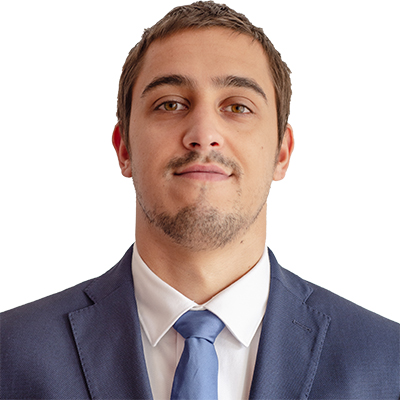
\includegraphics[width=\textwidth]{figures/david_2_linkdin.jpg} % Picture

    \vspace{2mm}

    \begin{skills}{Info}

    \nationality{Portuguese}

    \phone{+351 962 154 064}

    \email{davidmarques856@gmail.com}

    \faLinkedinSquare: \href{https://www.linkedin.com/in/djrmarques/}{/in/djrmarques}

    \faGithub: \href{https://github.com/djrmarques}{djrmarques}


    \vspace{3mm}
    \end{skills}
    % Here is the info

    \begin{skills}{Languages}

    \skillentry{Portuguese}{5}\\                                                                                                                                                   
    \skillentry{English}{5}\\
    \skillentry{German}{1}
    \end{skills}

    \begin{skills}{Programming}
    \skillentry{Python}{4}
    \skillentry{\LaTeX2}{4}
    \skillentry{Matlab}{3}
    \skillentry{HTML/CSS/JS}{2}
    \skillentry{Elisp}{2}
    \skillentry{R}{2}
    \skillentry{Scala}{2}
    \skillentry{Bash}{1}
    \skillentry{C}{1}
    \end{skills}

    \begin{skills}{Database}
    \skillentry{MySQL}{3}
    \skillentry{SQL Server}{3}
    \end{skills}

    \begin{skills}{VCS}
    \skillentry{Git}{3}
    \end{skills}

    \begin{skills}{Big Data}
    \skillentry{Spark}{3}
    \skillentry{Databricks}{2}
    \end{skills}

    \begin{skills}{Containers}
    \skillentry{Docker}{3}\\
    \end{skills}

    \begin{skills}{Hobbies}
    \unratedskill{Jiu Jitsu}\\
    \unratedskill{Reading}\\
    \unratedskill{Programming}\\
    \end{skills}


\end{minipage}&
\begin{minipage}[t][][t]{.65\linewidth}


  \begin{cvpart}{Experience}
  \experience{Data Scientist}{Apr/2019-Present}{\href{https://www.closer.pt/}{Closer Consulting}}\\
  Providing value from raw data and developing custom solutions for business challenges. Projects range from optimization, forecasting, model deployment and server migration and maintenance.
  \devskills{Python, Data Visualization, Data Cleaning, \\Metaheuristics Optimization, Machine Learning, \emph{SQL}, Git, Spark, Databricks}

  \end{cvpart}

  \begin{cvpart}{Projects}
    \experience{Production Plan Optimization}{Jun/2019-Nov/2019}{Closer Consulting}\\
    Metaheuristics based optimization to create a daily optimized production plan of 7 machines in order to maximize the total volume exported within the deadline.

    \experience{Transport Price forecasting}{Mar/2020}{Closer Consulting}\\
    Monthly prediction of transportation price.

    \experience{Spark Data Process}{Apr/2020}{Closer Consulting}\\
    Analysis and process of several millions of events produced by dataloggers with the respective geographical coordinates.
   

  \end{cvpart}


  % Education Bit
  \begin{cvpart}{Education}
    \experience{Mechanical Engineering Masters}{2011-2018}{Energy Department. \\ Instituto Superior T\'{e}cnico, Lisboa, Portugal. \\ Conclusion Grade: 15/20}

    Masters with focus on developing computational solutions and numerical methods for engineering problems.
    
    \experience{Master's Dissertation}{2018}{Smart ventilation controller\\Grade: 18/20
    }

   	Intelligent thermal comfort controller, capable of adapting to an office user's preference and autonomously managing the ventilation system. Learning system based on \emph{Reinforcement Learning.}
	\devskills{Python, \emph{SQL}, Linux, \LaTeX2, Git}
  \end{cvpart}

\end{minipage}
\end{tabular}
\end{document}

%%% Local Variables: 
%%% coding: utf-8
%%% mode: latex
%%% TeX-engine: luatex
%%% TeX-master: t
%%% End: 

